% !TeX root = ../main.tex

\section{Results}\label{sec:results}

Our thematic analysis of 13 interviews with crypto KOLs produces three sets of empirical findings aligned with the research questions. We interpret the recurring patterns and characteristics through the lens of SDT, providing conceptual grounding. Themes and subthemes are summarized in \Cref{tab:thematic-tree} with representative quotes and RQ mapping.

\subsection{RQ1: Motivational Factors for Crypto KOLs}\label{sec:rq1}

Our analysis reveals a blend of \emph{extrinsic} and \emph{intrinsic} motivators positioned along a continuum of relative autonomy (see Figure~\ref{fig:motivations}). Early entry is often encouraged by extrinsic factors (e.\,g., sponsorship income, visibility, access to projects). Sustained engagement is driven by more self-determined forms of motivation. Interpreted through SDT, KOLs describe trajectories in which external incentives are gradually internalised into self-endorsed values and identities organised around autonomy, competence, and relatedness. These qualitatively distinct forms of motivation are discussed below.% (see \Cref{tab:thematic-tree}).

\begin{figure*}[ht]
    \centering
    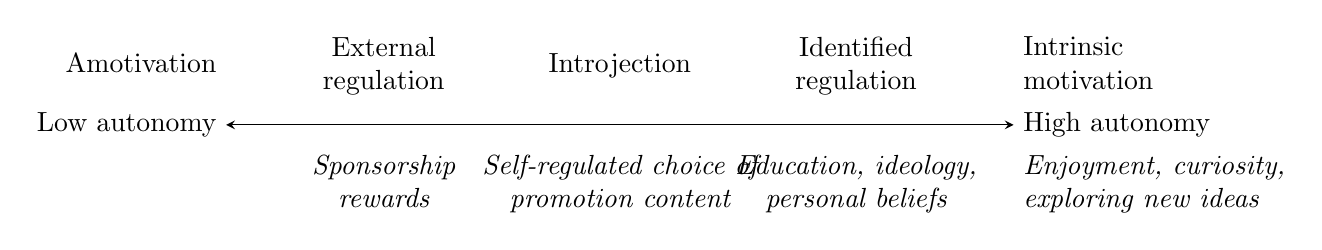
\begin{tikzpicture}[>=stealth]
        \draw[<->] (0,0.25) node[left]{Low autonomy} -- (10,0.25) node[right]{High autonomy};
        \node[left] at (0,1) {Amotivation\vphantom{Aq}};
        \node[align=center] at (2,1) {External\\regulation};
        \node[align=center] at (5,1) {Introjection};
        \node[align=center] at (8,1) {Identified\\regulation};
        \node[align=left, right] at (10,1) {Intrinsic\\motivation\vphantom{Aq}};
        \node[align=center,font =\itshape] at (2,-.5) {Sponsorship\\rewards\vphantom{Aq}};
        \node[align=center,font =\itshape] at (5,-.5) {Self-regulated choice of\\ promotion content\vphantom{Aq}};
        \node[align=center,font =\itshape] at (8,-.5) {Education, ideology,\\personal beliefs\vphantom{Aq}};
        \node[align=left, right,font =\itshape] at (10,-.5) {Enjoyment, curiosity, \\exploring new ideas\vphantom{Aq}};
    \end{tikzpicture}
    \caption{Motivational factors for crypto KOLs (\emph{in italics}) through the lens of SDT.}
    \label{fig:motivations}
    \Description{Motivational factors for crypto KOLs are mapped to SDT constructs and positioned along a continuum of relative autonomy (from low to high): sponsorship rewards (external regulation); self-regulated choice of promotion content (introjection); education, ideology, personal beliefs (identified regulation); and enjoyment, curiosity, exploring new ideas (intrinsic motivation).}
\end{figure*}

\noindent\textbf{Recalibrating incentives over time.} Consistent with SDT's account of internalisation, many KOLs recount a shift from externally regulated engagement (e.\,g., taking any sponsorship that pays) towards more self-regulated practices in which they reject misaligned opportunities in order to protect their autonomy and credibility:
\begin{quote}\itshape
``The more I progress in this space and the more mature it gets, I have less and less of an appetite to endorse crypto projects or coins.''
\textemdash{} KOL10
\end{quote}

\noindent\textbf{Credibility over cash.} Chasing money erodes credibility; autonomy sustains trust. Several participants explicitly describe self-imposed rules, such as declining projects they would not personally invest in, that prioritise long-term relatedness with their communities over short-term revenues.

\begin{quote}\itshape
``Even when a sponsor approaches me, I only cover it if I would recommend it to my community anyway. Otherwise, it undermines everything I've built.'' \textemdash{} KOL07
\end{quote}

\noindent\textbf{Education as a worthwhile mission.} Many participants emphasise an educational mission and community service, describing satisfaction from helping newcomers avoid mistakes and make sense of a complex, high-stakes ecosystem. This combination points to competence (mastery and explanation) and relatedness (care for an imagined community of followers).

\begin{quote}\itshape
``Educating people that they have to invest, otherwise they will be broke and poor, is the biggest motivation behind my work.'' \textemdash{} KOL01
\end{quote}

\noindent\textbf{Ideological commitment and mastery.} Interviewees link opinion leadership to personal values (e.\,g., critiques of incumbent finance, decentralisation ideals) and to curiosity and mastery in the fast-moving domain. These narratives foreground autonomy, as participants emphasise self-endorsed commitments to being ``at the forefront'' of technological change rather than simply chasing short-term gains.
Nine participants explicitly highlighted the dynamic nature of the crypto market as a field for impact:
\begin{quote}\itshape
``My motivation was to be at the forefront of this new technological revolution and have a chance to shape it.''
\textemdash{} KOL11
\end{quote}


\noindent\textbf{Key takeaway (RQ1).} Initial extrinsic incentives give way to more internalised motivations. As expertise and recognition grow, KOLs increasingly foreground autonomy (editorial independence and self-imposed standards), competence (continuous learning and translation work), and relatedness (educational stewardship of their communities) as reasons to remain active in high-risk crypto markets, even when this constrains short-term financial opportunities.

\subsection{RQ2: Defining Characteristics of Crypto KOLs}\label{sec:rq2}

We outline characteristics as themes aligned with SDT needs (cf. \Cref{tab:thematic-tree}), showing how autonomy, competence, and relatedness are enacted in high-risk crypto ecosystems and under algorithmic visibility constraints.

\noindent\textbf{Autonomy.}
Autonomy is often expressed in an individual's decision to take a deep dive into crypto- and blockchain-related topics and activities through a self-directed learning path. This process typically involves intensive reading, hands-on experimentation and asset trading, active browsing, and engaging in conversations with others in the community. Most participants described themselves as digital natives and reported technical, financial, or consulting backgrounds, which facilitated both their onboarding and continued interest in this field. Over time, few KOLs have introduced premium content and community memberships as strategies to achieve greater (financial) autonomy and to transition from platform-controlled monetisation to community-driven value creation and exchange.

Once excellence in subject matter and a follower base are secured, KOLs place a high value on the freedom to articulate their own perspectives and share their opinions with a broader audience:
\begin{quote}\itshape
``[As a KOL], you have the influence of letting people know what you think. I can curate an official crypto narrative and put it in the way I feel like it's the right way.'' \textemdash{} KOL01
\end{quote}

Autonomy is also expressed through self-imposed policies and guiding principles that many of the interviewed participants developed to govern their content creation and sponsorship decisions. In particular, crypto KOLs tend to be highly-selective, prioritising value-adding, meaningful, and solution-oriented media publications. By contrast, non-serious or controversial posts are perceived as harmful to authentic self-expression:
\begin{quote}\itshape
``I don't like putting out content to entertain.'' \textemdash{} KOL10
\end{quote}

In rare cases, the autonomy of crypto KOLs extends beyond individual self-expression towards actively shaping the broader institutional environment. By positioning themselves as intermediaries between regulators and the crypto community, KOLs demonstrate both autonomy and competence, thereby aligning their self-endorsed values with influence at the systemic level:
\begin{quote}\itshape
``When it comes to crypto regulation, we lead regulators down a path that is sustainable, because they are often lacking technological know-how. We exert some influence on the ecosystem---not so much on the masses, but indirectly through contributing to the formation of regulation.'' \textemdash{} KOL11
\end{quote}

%Many participants articulated explicit independence policies (e.g., disclosure, no pay-to-post, editorial control). Guarding against sponsor interference was framed as essential to maintaining trust and long-term reputation.

\noindent\textbf{Competence.}
Crypto KOLs tend to maintain an enduring commitment to developing highly-specialized expertise, often by concentrating on a specific domain or a narrower subset of topics (e.\,g., financial advisory, the dynamics between macroeconomics and cryptocurrencies, crypto-asset taxation, prediction or regional markets). Their competence is primarily demonstrated through the ability to simplify and communicate complex issues in an accessible, timely, and transparent manner:

\begin{quote}\itshape
``If you want to be trusted, you have to be able to articulate quite complicated things in a relatively simple fashion, because blockchain [technology] is a multidisciplinary, quite complicated matter. Nobody can profess you to know it all, but you have to be able to communicate well about all the little bits and pieces that you slice out per your preference. '' 
 \textemdash{} KOL08
\end{quote}

Some KOLs, in particular those offering  advisory services, further perceive themselves as curators and interpreters of financial information, synthesizing multiple sources (e.\,g., on-chain and market data, technical documentation, analytical reports, research publications) and data points to provide clarity and actionable guidance for their followers. These skills distinguish crypto KOLs from other influencers, as their authority is grounded not in popularity, entertainment or promotion value, but in demonstrable expert knowledge, analytical rigour, and the capacity to translate highly technical content into practical insights in a volatile, high-risk environment. In SDT terms, competence is experienced not only as private mastery but as the ability to help others navigate complex infrastructures without resorting to hype.

Beyond knowledge creation and dissemination, crypto influencers invest considerable effort into proactive management of their reputation and personal image. As KOL08 described, maintaining their \emph{social reputation} involves  transparent communication, careful selection of topics and partnerships, and adherence to self-imposed ethical standards. Ultimately, a KOL's reputation serves as a signal of expertise, reinforcing the credibility and trustworthiness of the online content they share.

In terms of content creation strategies, crypto KOLs note that blending educational  materials and investment ideas with emotion-triggering narratives (e.\,g., personal stories, analogies, or provocative framings) elicit the strongest responses from their audiences. This balancing act between education and engagement also mirrors the competitive dynamics of the broader influencer market, in which celebrities and influential figures compete for visibility and audience attention~\cite{franck2019economy}:

\begin{quote}\itshape
``There is a fight for attention, but it's not hostile; people focus on a topic and aim to attract attention through quality content rather than by undermining others.'' 
 \textemdash{} KOL11
\end{quote}
%KOLs triangulate across technical documentation, on-chain data, and peer review to reduce uncertainty. They translate complexity into accessible narratives without oversimplifying, and routinely update analyses in response to new evidence. This combination of depth and clarity differentiates them from purely promotional voices.

\noindent\textbf{Relatedness.} 
Given the positive effect of interpersonal connections on human well-being~\cite{Reis2000DailyWellBeing}, crypto KOLs actively pursue a sense of belonging and social recognition through their online and offline interactions with like-minded followers. Some invest considerable effort into community building and mutual support, striving to cultivate online environments that foster connectedness, shared purpose, and collective enthusiasm. Others adopt a more conservative approach, prioritising in-person connections and conference participations while using social media primarily as a post hoc amplifier of their offline activities. 

Building on these modes of interaction, our participants also highlighted the importance of strategically navigating through various social media platforms to maintain their influence and visibility. Crypto KOLs differentiate their use of platforms, leveraging Instagram as a medium for outreach and audience acquisition, while employing YouTube for extended content formats with in-depth know-how:
\begin{quote}\itshape
``On YouTube, the community is usually smaller but the content is longer, more binding, and has a strong opinion-shaping effect. By contrast, on X (formerly Twitter) or Telegram the exchanges are made up of short, regular inputs signals that quickly fade away. If people actually engage with YouTube, you have a much stronger influence on them than through these fleeting messages.''  \textemdash{} KOL11
\end{quote}
Despite its declining popularity, X (formerly Twitter) continues to serve as an important channel for many of the interviewed participants, primarily due to its established role in the ecosystem, the concentration of crypto-interested communities, and networking opportunities. At the same time, KOLs increasingly adopt Telegram and Discord, which are regarded as platforms offering more direct community interaction, private modes of engagement, and an access to niche audiences. Many interviewees described TikTok as the least favourable platform, largely due to its popularity among young audiences and the frequent promotion of meme coins and speculative projects. Avoiding such environments was portrayed as a deliberate choice, allowing the interviewed KOLs to protect their professional credibility. 

While Telegram, Discord, and X are generally associated with instant and high-volume exchanges, some interviewees emphasised that LinkedIn fulfils a different role within their communication strategies. In particular, LinkedIn distinguishes itself through its perceived professionalism and the prevalence of authentic, non-fake accounts. For many KOLs, maintaining a presence on LinkedIn complements their credibility-building strategies, as it aligns with their aspiration to be recognised as trustworthy experts rather than mere entertainers. Furthermore, LinkedIn enables crypto KOLs to reach a different audience (e.\,g., companies, entrepreneurs, and developers) and engage in more high-quality discussions compared to the community-driven spaces such as Telegram or Discord. At the same time, several participants noted that LinkedIn's dynamic algorithms require continuous adaptation of content and framing to sustain impressions and ensure that their messages reach intended audiences, highlighting how platform-level engagement metrics shape day-to-day communication choices.

Finally, beyond the platform diversification, KOLs also employ specific communicative practices to reinforce their credibility and strengthen audience ties. Beyond consistent publishing crypto-related materials,  participants described a range of dialogic interactions as crucial for sustaining trust. Common practices include replying to comments, engaging in respectful debates, hosting live Q\&A sessions, and organising webinars and podcasts. Such interactive formats invite feedback and collective sensemaking, thereby strengthening bonds with online communities.

%\begin{quote}\itshape
%"If a project wants pre-approval of my script, that's a red flag. I need full editorial control or I walk away." \textemdash{} KOL-03 (Researcher/Commentator)
%\end{quote}

\noindent\textbf{Key takeaway (RQ2).} Authoritative KOLs align autonomy (independence, self-imposed rules), competence (specialised expertise, translation, curation, reputation), and relatedness (community stewardship, dialogic practices, platform navigation) while selectively engaging with platform algorithms and attention dynamics. They differentiate between channels, avoiding spaces that normalise meme-coin speculation and tailoring formats to sustain influence and credibility under shifting visibility metrics.

\subsection{RQ3: Ethics, Social Responsibility, and Community}\label{sec:rq3}

Our participants articulated a nuanced sense of ethical duty and community accountability in their roles as blockchain influencers. They acknowledged that their communication can meaningfully sway token prices and investment sentiment and therefore requires careful self-regulation and transparent disclosure in thin, speculative markets where low-cap tokens can move sharply on limited liquidity. Read through SDT, these accounts show how autonomy (self-imposed rules), competence (bounded claims and careful translation), and relatedness (care for followers' outcomes) underpin KOLs' ethical self-understandings.

\noindent\textbf{Self-restraint and responsible promotion.} Several KOLs recognise that their ability to move markets obliges restraint.  KOL01 explained that their follower count gives them power to influence low-cap tokens and thus obliges them to avoid fraudulent practices:  
\begin{quote}\itshape
``It's definitely my responsibility to not recklessly inside trade.  I noticed I can move an asset that has a market cap of 200{,}000~(USD)—I can move it up $10\text{--}20\%$ easily.''  \textemdash{} KOL01
\end{quote}
KOL03 similarly reflected on the past episode in which they promoted an adult-content project that turned into a publicity disaster.  They now refuse requests to shill tokens\footnote{In the context of cryptocurrency discourse, \emph{to shill} denotes the act of aggressively or uncritically promoting a digital asset, often with undisclosed financial incentives or conflicts of interest. The term carries a negative connotation, implying manipulative or deceptive endorsement rather than impartial evaluation.}, noting that short-term gains would damage their reputation:  
\begin{quote}\itshape
``I have still sometimes requests \ldots would we give you some token?  Could you please push a bit?  I don't, because this actually harms my image.''  \textemdash{} KOL03
\end{quote}
KOL9 and KOL11 avoid direct market commentary altogether.  The former stated that their organisation only posts after results and ``\emph{don't shill tokens, we educate users about the projects},'' while the latter emphasised that as a regulatory expert they refrain from opining on whether particular coins are scams, positioning themself as a neutral actor rather than a promoter. Taken together, these practices exemplify self-regulation: KOLs voluntarily constrain their own promotional options to protect both their reputations and their communities' financial well-being.

\noindent\textbf{Transparency, disclosure, and honesty.} Most interviewees describe strict disclosure norms.  KOL10 recounted that during the NFT boom they labelled every sponsored thread as paid content and that this transparency protected them from backlash when projects underperformed: 
\begin{quote}\itshape
``I would disclose that, hey, this is paid \ldots and it would have market impact \ldots I never got any blame, because if you are upfront and honest \ldots had I not disclosed, I probably would have gotten blamed.'' \textemdash{} KOL10
\end{quote}
They added that they have ``less and less of an appetite'' to recommend specific assets and now stick to high-level portfolio allocations, holding themself to ``a much higher standard.''  KOL2 characterised themself as ``too honest'' and noted that they always warn followers about risks, even though ``people always blame you as an influencer'' regardless of the outcome.  KOL12, representing a venture fund, stated that they will always disclose when a post concerns a portfolio company: 
\begin{quote}\itshape
``We will always write a disclaimer … you have to disclose that you are an investor \ldots this is part of our policy.''  \textemdash{} KOL12
\end{quote}
These statements underscore a shared conviction that undisclosed conflicts of interest violate community norms, yet they also reveal tensions between transparency and accountability: even when disclosures and risk warnings are explicit, influencers anticipate being blamed if followers incur losses.

\noindent\textbf{Community norms and trust building.} Influencers link ethical practice to long-term relationship building.  KOL08 argued that trust hinges on the ability to translate complex concepts without feeding speculation:  
\begin{quote}\itshape
``If you want to be trusted, you have to be able to articulate quite complicated things in a relatively simple fashion \ldots I explicitly never engage in any sort of commentary around the markets.''  \textemdash{} KOL8
\end{quote}
KOL9 emphasised authenticity through ``\emph{meeting people in real life}'' and being ``super doxxed'' in order to show that they are ``really honest'' about what they do.  KOL13 recalled that leaving a traditional finance job was partly motivated by the sector's openness; they highlighted that in the early days ``\emph{everyone was helping each other}'' and that they have ``not seen that good of a knowledge transfer in Web2.''  Such accounts portray a community that values mutual support and education over hype and illustrates how relatedness is sustained through mutual visibility and knowledge sharing.

\noindent\textbf{Managing controversies and reflective practice.} Participants describe strategies for navigating controversies and learning from mistakes.  When asked about a controversial presale, KOL10 explained that they chose not to respond publicly because defending themself would only inflame anger.  KOL3's reflection on their failed promotion taught them to decline paid advertisements and to prioritise social impact over money.  They summarised their credo succinctly:  
\begin{quote}\itshape
``Trust is the most important thing.  How can I promote the trust technology when I cannot be trusted \ldots I don't do any paid ads anymore \ldots it harms my image.''  \textemdash{} KOL3
\end{quote}
KOL13, who regularly publishes long-form research threads, observed that even accurate analyses can be misconstrued as buy signals.  They now avoid validating their own calls and resist the role of a prognosticator:  
\begin{quote}\itshape
``I don't think I've ever revalidated my own thesis $\ldots$ I don't want to end up being a KOL on Twitter at all.  I want to have like 300–400 followers $\ldots$ because then I'll be doing back and forth with [researchers], and people would realize \ldots that's the contradiction we live in---people don't want me to make sense, they want me to give advices.''  \textemdash{} KOL13
\end{quote}
They added that even prominent figures ``\emph{not even Vitalik Buterin\footnote{Vitalik Buterin is a Russian–Canadian programmer best known as the co-founder of Ethereum, one of the most widely used blockchain platforms.} \ldots not even the best traders}'' can reliably pick winning tokens; thus ``\emph{everyone gets to start from the same line},'' reinforcing the need for humility. Such reflections illustrate ongoing internalisation of ethical standards, as KOLs adapt their practices to align more closely with their self-perception of being trustworthy educators rather than forecasters.

\noindent\textbf{Key takeaway (RQ3).} KOLs position themselves as custodians of norms in high-risk, attention-driven markets, enacting credibility through four self-determined practices: (i)~\emph{self-regulation and voluntary constraint}, whereby KOLs decline misaligned sponsorships and impose personal rules on promotion; (ii)~\emph{bounded epistemic competence}, acknowledging limits and avoiding prognostication; (iii)~\emph{accountability}, cultivating long-term trust through transparent disclosure; and (iv)~\emph{reflexive self-correction}, learning from failures and continuously reassessing practices. These practices reframe credibility as an ongoing, ethically enacted performance rather than possessing a set of static credentials.
